\begin{FPfigure}

\begin{center}
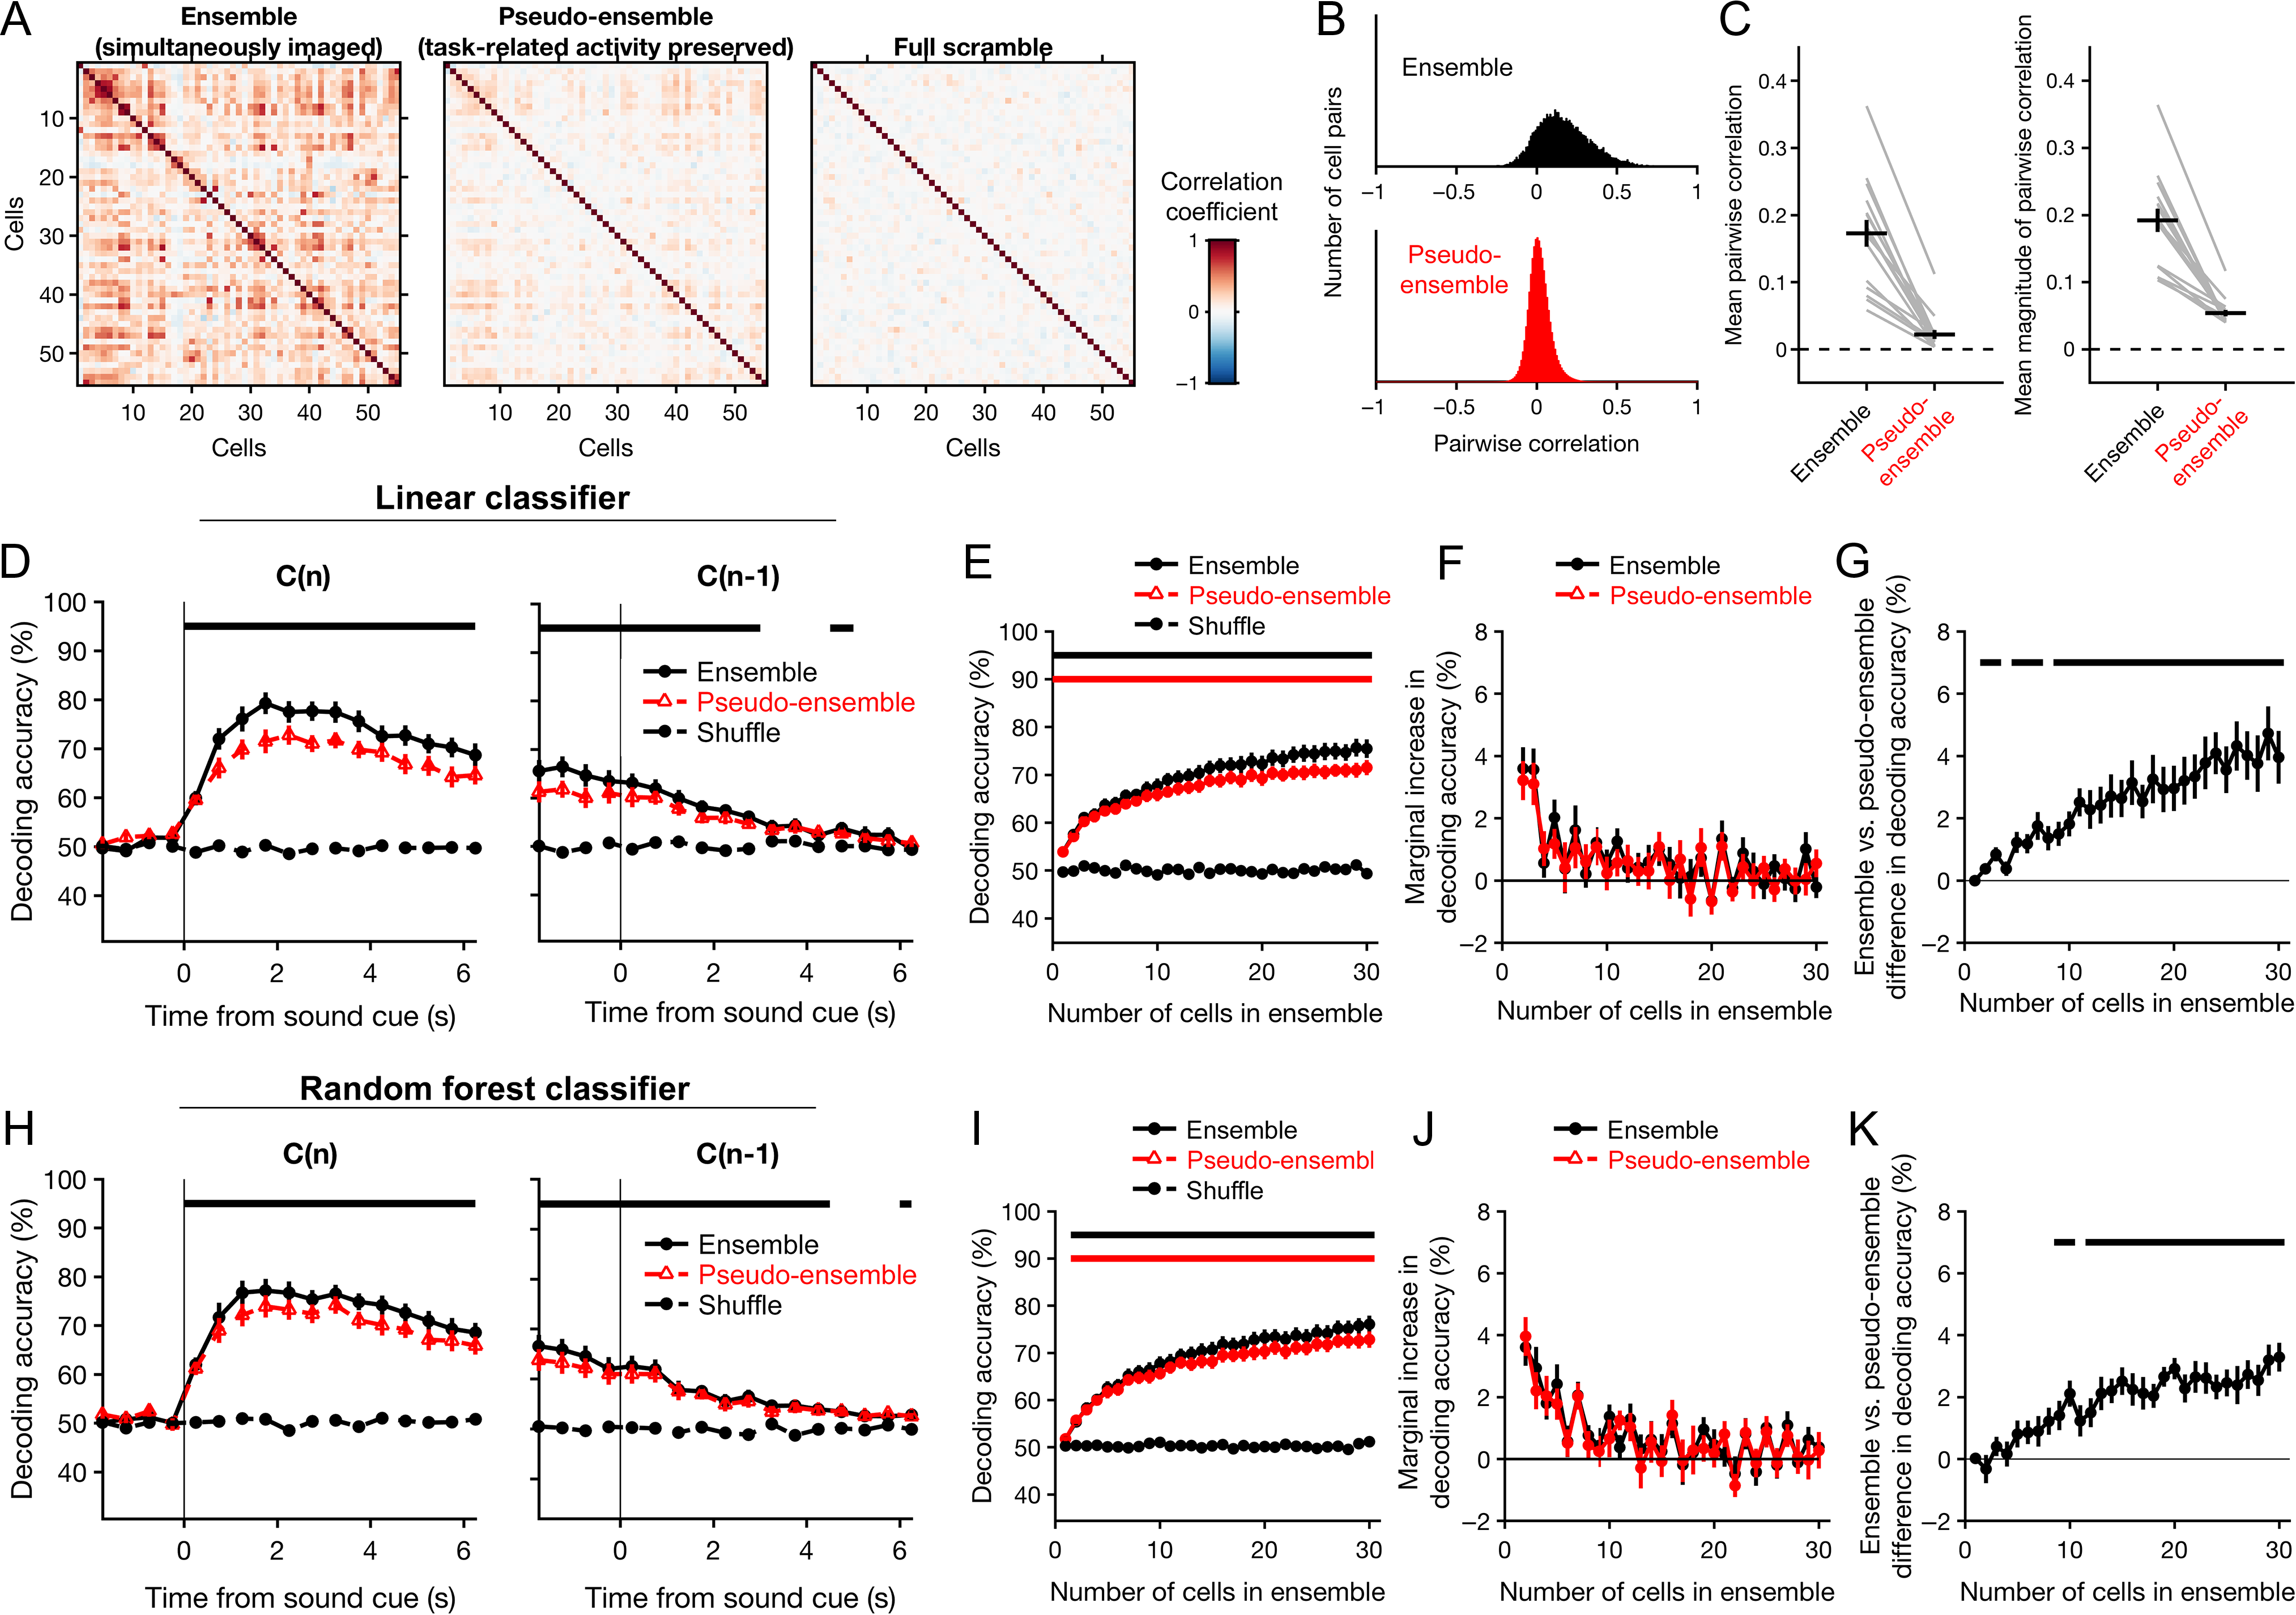
\includegraphics[width=\textwidth]{Figures/CC_fig7.png} 
\small{Figure \ref{fig:CC_fig7}: Decoding advantage of simultaneous recording increased with ensemble size.}
\end{center}

\caption[Decoding advantage of simultaneous recording increased with ensemble size]
{Simultaneous recording imparted a decoding advantage that increased as a function of ensemble size. The accuracy of decoding choices from the activity of simultaneously imaged ensembles of neurons was compared to that of pseudo-ensembles in which simultaneity was disrupted by shuffling the activity traces from each neuron across trials in which the same choice was made. Only correct trials resulting in a single reward were used for this analysis. Classification accuracy was tested using Monte Carlo cross-validation (repeated random subsampling). Chance-level accuracy was determined by testing classifiers constructed using shuffled choices. (A) Pearson correlation matrix for all cells from one example session, under three conditions: with simultaneity preserved (‘ensemble’), after shuffling across trials with the same chosen action (‘pseudo-ensemble’), and after shuffling across trials irrespective of chosen action (‘full scramble’). Correlations were estimated from cellular fluorescence averaged over the interval from 2 to 4 s following cue onset. (B) Histogram of the Pearson correlation coefficients estimated for all pairs of cells imaged in all experiments, using simultaneous ensembles (top) and pseudo-ensembles (bottom). (C) Mean pairwise correlation (left), and pairwise correlation magnitude (right) across all sessions. Gray lines, means from individual sessions. Black crosshairs, $grand mean \pm SEM$. (D) Performance of decoders based on linear discriminant analysis, plotted as a function of time for single-reward trials (left), or trials in which the previous outcome was a single reward (right). Accuracy of ensemble classifiers (black circles) is overlaid with that of pseudo-ensemble classifiers (red triangles) for visual comparison. Black dashed line, chance-level accuracy. (E) Decoder performance as a function of the number of cells used to decode the chosen action. Performance of ensemble (black circles) and pseudo-ensemble (red triangles) classifiers was estimated as the mean classification accuracy over the interval from 2 to 4 s following cue onset in single-reward trials. The number of cells was varied from 1 to 30 by drawing cells randomly from the full ensemble or pseudo-ensemble without replacement. Black dashed line, chance-level accuracy. Horizontal bars, bins in which ensemble (black, upper bar) or pseudo-ensemble (red, lower bar) classifiers performed significantly better than chance ($P < 0.05$, Wilcoxon signed-rank test). (F) Marginal percentage point change in decoding accuracy, plotted as a function of ensemble size for ensembles (black) and pseudo-ensembles (red). (G) Difference in accuracy of the ensemble and pseudo-ensemble decoders shown in E–F, plotted as a function ensemble size. Black horizontal bars, bins in which the accuracy of ensemble and pseudo-ensemble classifiers differed significantly ($P < 0.05$, Wilcoxon signed-rank test). (H–K) Same as D–G for random forest classifiers. Data in D–K are presented as $mean \pm SEM$.} 
\clearpage
\label{fig:CC_fig7}
\end{FPfigure}